\section{Ziel}
    In diesem Versuch sollen die Topologien verschiedener Strukturen im Micrometerbereich sowie die von Speicherdiscs wie CD, DVD und Blu-Ray untersucht werden. Dazu wird die Methode der \textit{atomic force
    microscopy} (AFM) verwendet, die auf der Auslenkung einer wenigen Nanometer großen Spitze aufgrund der Wechselwirkung zwischen dieser und den Oberflächenatomen basiert.    
    
\section{Theoretische Grundlagen}
    \subsection{Messprinzip}
        Das klassische Messprinzip der AFM ist in Abbildung \ref{fig:prinzip} visualisiert. Eine \textbf{Messspitze} (\textit{Probe Tip}), die an einem \textbf{Cantilever} befestigt ist, wird auf eine 
        Entfernung von wenigen Angström bis einigen \SI{100}{\nano\metre} and die Probenoberfläche gebracht. Die zwischen der Messspitze und den Oberflächenatomen wirkende Kraft resultiert aus verschiedenen
        distanzabhängigen \textbf{Wechselwirkungen} und wird auf den Cantilever übertragen. Verschiedene \textbf{Detektionssysteme} erlauben es die wirkende Kraft über den Cantilever zu messen und so den 
        Abstand zwischen Messspitze und Oberfläche zu bestimmen. In Kombination eines elektronischen Feedback-Loops und \textbf{Piezoelementen}, die die Probe relativ zur Messspitze in x-, y- und z-Richtung
        verschieben können, ist es möglich diese Abstandsmessung auf der gesamten Probe durchzuführen und so ein Höhenprofil der Oberfläche zu ermitteln. Da je nach Distanz verschiedene Kräfte dominieren und
        der Feedback-Loop es auch ermöglicht auf verschiedene Weise über die Probe zu rastern, kann die AFM in mehreren \textbf{Messmodi} betrieben werden.

        \FloatBarrier

        \begin{figure}[h]
          \centering
          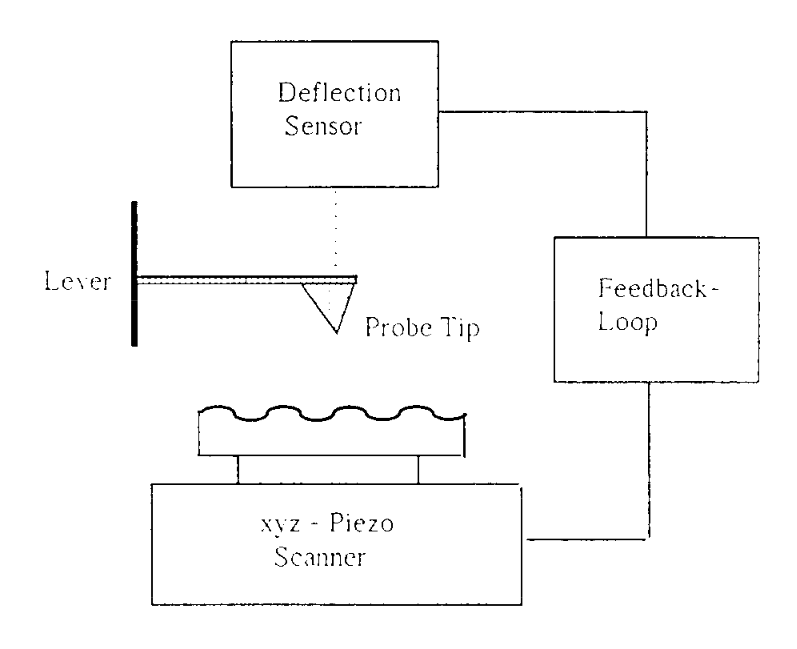
\includegraphics[width = 0.4\textwidth]{pictures/prinzip.png}
          \caption{asd}
          \label{fig:prinzip}
        \end{figure}
    
        \FloatBarrier


      \subsection{Wechselwirkungen}

        \subsubsection{Spitze - Oberfläche}
          Zur Vermessung des Höhenprofils der Oberfläche wird die distanzabhängige Kraft zwischen Messspitze und Oberfläche genutzt. Das zugehörige Potential wird als Lennard-Jones-Potential 

          \begin{equation*}
            \text{U(R)} = 4\text{U}_0 \left[ \left(\frac{\text{R}_{\text{a}}}{\text{r}}\right)^{12} - \left(\frac{\text{R}_{\text{a}}}{\text{r}}\right)^{6} \right]
          \end{equation*}

          angenähert, das einen positiven und demnach repulsiven Anteil und einen attraktiven Anteil besitzt, und in Abbildung \ref{fig:LJ} (a) mitsamt der resultierenden Kraft (b) und dem zugehörigen
          Kraftgradienten (c) dargestellt ist.

          \FloatBarrier

          \begin{wrapfigure}{L}{6cm}
            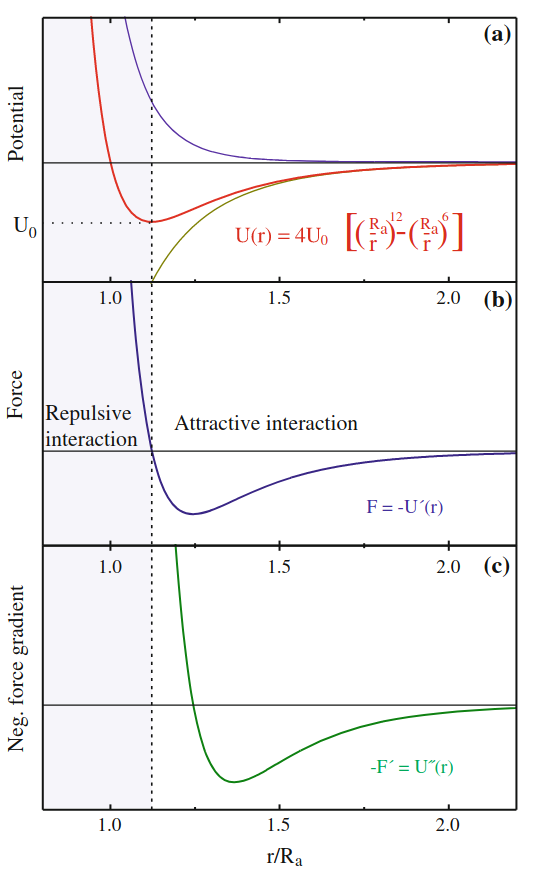
\includegraphics[scale = 0.3]{pictures/LJ.png}
            \caption{hdf}
            \label{fig:LJ}
          \end{wrapfigure}

          \FloatBarrier

          Das Potential setzt sich aus verschiedenen Wechselwirkungen zusammen, die für unterschiedliche Entfernungen dominant sind.\newline 
          Der attraktive Bereich für Abstände über \SI{1}{\nano\metre} resultiert hauptsächlich aus den \textit{Van-der-Waals-Kräften}. Diese beschreiben die Anziehung zweier eigentlich neutraler Atome durch die 
          spontane Entstehung von fluktuierenden Dipolen. Entsteht in einem Atom eine 
          spontaner Dipol, wird im benachbarten Atom ebenfalls ein Dipol induziert und die Atome ziehen sich an. Das zugehörige Potential fällt mit $\frac{1}{\text{r}^6}$ ab und ist demnach langreichweitig. 
          Deswegen wechselwirkt nicht nur das vorderste Atom der Spitze mit der Oberfläche, sondern auch dahinterliegende.\newline

          Für Distanzen unter \SI{1}{\nano\metre} kommt es zu chemischen Bindungen, bei denen die Orbitale der beteiligten Atome hybridisieren. Führt dies zu einer Verringerrung der Gesamtenergie wirken diese 
          Bindungen attraktiv. Erhöht sich die Gesamtenergie wirken die Bindungen repulsiv.

          Für Distanzen unter \SI{1}{\angstrom} kommt es zu stark repulsiven Wechselwirkungen. Die dominante Abstoßung folgt aus dem Pauli-Prinzip, nach dem zwei Elektronen mit dem selben Spin nicht den selben 
          Zustand besetzen dürfen. Bei sehr geringen Distanzen führt der Überlapp der Orbitale dazu, dass Elektronen in höhere unbesetzte Bänder ausweichen müssen. Dies führt zu einer starken Erhöhung der 
          Gesamtenergie und somit zu einer repulsiven Kraft. Zusätzlich kann auch Coulombabstoßung zwischen den Kernen auftreten, wenn diese nicht komplett durch ihre Elektronen abgeschirmt sind.

          Falls zwischen der Spitze und der Oberfläche eine Potentialdifferenz vorliegt, kommt es zusätzlich zu elektrostatischen Kräften. Diese können jedoch vermieden werden, indem die Potentialdifferenz durch
          das Anlegen einer entsprechenden Spannung kompensiert wird.\newline

        
        \subsubsection{Cantilever - Spitze - Oberfläche}

          \FloatBarrier

          \begin{wrapfigure}[28]{L}{5cm}
            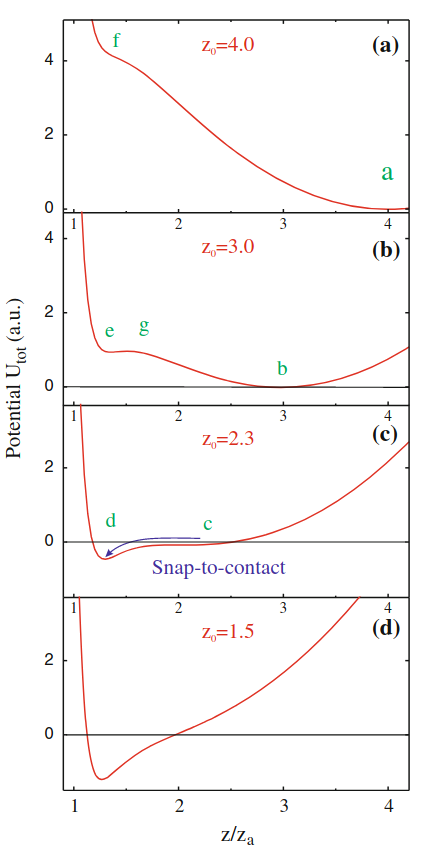
\includegraphics[scale = 0.3]{pictures/pot_contact.png}
            \caption{hdf}
            \label{fig:pot_contact}
          \end{wrapfigure}

          \FloatBarrier

          In einem AFM-Aufbau ist die Spitze an einem Cantilever befestigt, der als Feder fungiert und so ebenfalls Einfluss auf die Gesamtkraft nimmt. Nach dem Hook'schen Gesetz ergibt sich eine Kraft 
          
          \begin{equation*}
            \text{U}_{\text{F}} = \frac{1}{2} \text{k} \left(\text{z} - \text{z}_0\right)^2 \, ,
          \end{equation*}
          
          die linear in der Auslenkung z um eine Ruheposition z$_0$ und proportional zur Federkonstante k ist. Die Auswirkungen dieser Kraft lassen sich über Abbildung \ref{fig:pot_contact} erklären, in der 
          das Federpotential, für verschiedene Ruheposition auf das Lennard-Jones-Potential addiert, dargestellt ist. Wenn der Cantilever weit von der Oberfläche entfernt ist (a), besitzt des Potential ein 
          Minimum an der Ruheposition des Cantilevers. Wird der Cantilever mitsamt der Spitze angenähert (b), entsteht ein zweites lokales Minimum. Dieses liegt nah an der Oberfläche und ist von der Ruheposition
          nicht zu erreichen, da ein Maximum die beiden Minima trennt. Ab einer Grenze geht dieses Maximum in einen Sattelpunkt über und ein Übergang in das zweite Minimum wird möglich. Dieser Übergang wird als
          snap-to-contact bezeichnet und beschreibt einen Endzustand, in dem die abstoßenden Kräfte ein weiteres Annähern an die Probe verhindern. 





        \subsubsection{Kraft-Distanz-Kurven}

          Aus den gegebenen Potentialverläufen lässt sich begründen, welche Kraft auf das System aus Messspitze und Cantilever wirkt, wenn es an die Oberfläche herangebracht oder entfernt wird. Dieses Verhalten
          wird in Force-Distance-Curves dargestellt, die die Kraft für einen vollen Zyklus aus Annäherung und Entfernung gegen den Abstand auftragen. Charakteristisch für den Annäherungsprozess ist zunächst
          eine Kräftefreiheit, bis zu einem plötzlichem negativem Kraftgradienten, der einer Anziehung zur Probe entspricht und aufgrund des snap-to-contacts auftritt. Da mit diesem Schritt die Messspitze auf 
          der Oberfläche aufliegt, steigt die Kraft bei weierer Annäherung linear bis zu einem Maximum, bei dem das Annähern gestoppt wird. Wenn das Messsystem entfernt wird, sinkt die Kraft analog zu ihrem 
          vorherigen Anstieg. Bis die wirkende Kraft bei dem selben Abstand wieder ihr Vorzeichen wechselt.


          \FloatBarrier

          \begin{figure}[h]
            \centering
            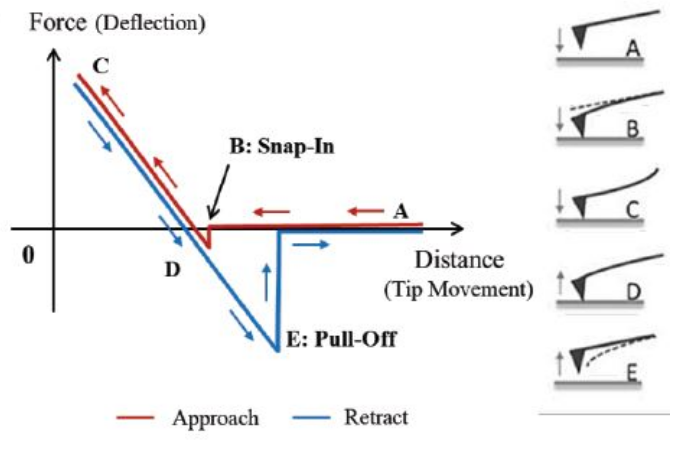
\includegraphics[width = 0.4\textwidth]{pictures/forcedist.png}
            \caption{asd}
            \label{fig:forcedist}
          \end{figure}
        
          \FloatBarrier






      \newpage


      \subsection{Messspitze und Cantilever}
        Die Messspitze und der Cantilever gehören zu den Hauptbauteilen, da auf sie die Kraft wirkt beziehungsweise sie die Kraft weitergeben, die später Rückschlüsse auf die Topologie der Oberfläche geben soll.
        Deswegen müssen sie spezielle Eigenschaften besitzen, die in der Anwendung auch unterschiedliche Messmodi ermöglichen können.

        \subsubsection*{Messspitze}
          Die Messspitze ist das Bauteil, das der Oberfläche am nähesten kommt und tatsächlich mit ihr wechselwirkt. Eine unendliche glatte Oberfläche könnte mit einer stumpfen Spitze vermessen werden. Wenn
          die Oberfläche jedoch nicht glatt ist und distinkte Hindernisse gemessen werden sollen, kommen neue Anforderungen auf die am besten über die in Abbildung \ref{fig:defekte} abgebildeten Messdefekte
          zu begründen sind. In Abbildung \ref{fig:defekte} a) und b) ist zu erkennen, dass eine zu stumpfe Spitze womöglich nicht in der Lage ist zu steile Objekte zu erkennen. Das gemessene Profil (rot) ist
          immer eine Faltung aus dem Profil der Spitze und dem der Oberfläche. Um nun kleine und steile Signale zu detektieren, muss die Spitze steiler zusammenlaufen als der steilste Gradient an der 
          Probenoberfläche und dünner sein, als das kleinste Objekt. In der Anwendung sind Spitzendurchmesser im einstelligen Micrometerbereich und Krümmugsradien von wenigen Nanometern möglich. Eine weitere
          Quelle für Defekte sind die in Abbildung \ref{fig:defekte} zu sehenden Beulen an der sonst flachen Spitze. Diese müssen unbedingt vermieden werden, da sie nicht vorhandene Strukturen an der Oberfläche
          im Höhenprofil erzeugen. 
        
          \FloatBarrier

          \begin{figure}[h]
            \centering
            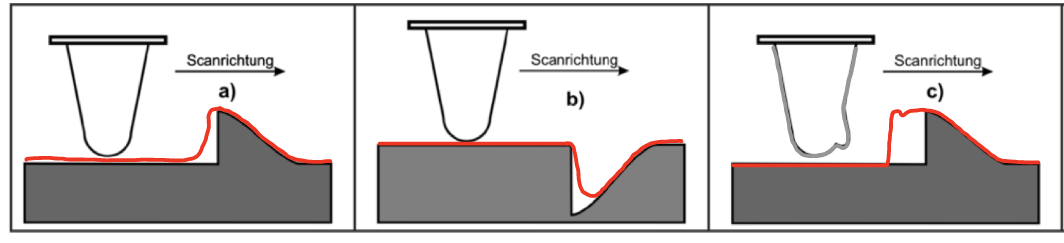
\includegraphics[width = 0.8\textwidth]{pictures/defekte.png}
            \caption{asd}
            \label{fig:defekte}
          \end{figure}
        
          \FloatBarrier

        
          \newpage
        \subsubsection*{Cantilever}
          Der Cantilever nimmt die auf die Messspitze wirkende Kraft auf, indem er sich verbiegt. Um diese Verbiegung zu Kraftmessung gut detektieren zu können, muss auch der Cantilever bestimmte Eigenschaften
          besitzen. Diese sind besonders an verschiedene Messmodi gekoppelt. Da der Cantilever sehr geringe Kräfte im Bereich von $10^{-9} \si{\newton}$ detektierbar machen muss, soll er sich bereits bei diesen
          Kräften genügend auslenken. Hier werden Federkonstanten von ca. $10 \si{\newton\per\metre}$, die detektierbare Auslenkungen im Angström Bereich erlauben. Zusätzlich soll der Cantilever eine  
          Resonanzfrequenz >> $10 \si{\kilo\hertz}$ besitzen, um in dynamischen Messungen, bei denen sich der Cantilever bewegt, die Messgeschwindigkeit zu erhöhen. Aufgrund der geringen Federkonstante folgt
          aus der Anforderung an die Resonanzfrequenz

          \begin{equation*}
            \omega_{\text{Res}} = \sqrt{\frac{\text{k}}{\text{m}}}
          \end{equation*}

          eine sehr geringe Masse des Cantilevers im Microgrammbereich.


      \newpage
      \subsection{Detektionssysteme}
          In diesem Versuch soll die Zusammensetzung von neun Würfeln innerhalb einer 3x3-Würfelebene bestimmt werden. Dazu wird der Würfel aus verschiedenen Richtungen bestrahlt und die transmittierte 
          Intensität gemessen. In eine Richtung i ergibt sich diese zu


      

      \newpage
      \subsection{Messmodi}
          In der AFM können verschiedene Messmodi genutzt werden, um unterschiedliche Eigenschaften der Oberfläche oder auch allgemeiner unterschiedliche Oberfläche zu untersuchen. Grundlegend wird dabei 
          zwischen statischen und dynamischen Messungen sowie Messungen mit oder ohne Kontakt zur Oberfläche unterschieden. 

          Wenn die Messspitze in Kontakt zur Oberfläche steht, liegt der Abstand zwischen Messspitze und Oberfläche im repulsiven Bereich des Potentials unter \SI{10}{\nano\metre} und die Messspitze wird von 
          der Oberfläche weggedrückt. In diesem Modus lässt sich die Topologie der Oberfläche beinahe atomar auflösen. Ein zusätzlicher Vorteil dieses Modus ist, dass die Messspitze durch flüssige 
          Oberflächenkontaminationen hindurchmisst. Der konstante Kontakt zur Oberfläche birgt die Gefahr des Abbrechens der Messspitze oder Beschädigung der Oberfläche. Messung im \textit{contact mode}
          können statisch und dynamisch durchgeführt werden. In statischen Messungen wird der Cantilever durch die wirkende Kraft verbogen und diese Biegung gemessen. Es kann entweder die Höhe der Messspitze
          über der Oberfläche konstant gehalten und die Änderung der Biegung gemessen werden (\textit{constant height}) oder die Biegung  und demenstprechend auch die Kraft konstant gehalten werden, indem
          der Abstand zwischen Messspitze und Oberfläche durchgehend nachreguliert wird (\textit{constant force}). In dynmaischen Messungen schwingt das System aus Cantilever und Messspitze mit dessen 
          Resonanzfrequenz von einigen kHz. Nähert sich die Spitze nun mit jeder Schwingperiode stark genug an die Oberfläche an, dass repulsive Kräfte auftreten, wird die AFM im \textit{tapping-mode}
          betrieben, der die dynamischen Messungen mit Oberflächenkontakt beschreibt. Die Distanz wird aus der Erhöhung der Resonanzfrequenz durch die abstoßende Kraft berechnet. 
          
          
          Liegt die Entfernung zwischen Messspitze und Oberfläche zwischen \SI{10}{\nano\metre} und \SI{10}{\micro\metre}, stehen beiden nicht in Kontakt (\textit{non contact mode}) und es wirkt eine 
          attraktive Kraft. Da kein Kontakt vorliegt, ist die Oberfläche in diesem Modus vor Beschädigung geschützt. Analog zum \textit{contact mode} kann auch hier zwischen statischen und dynamischen 
          Messungen unterschieden werden. Da die Kraft nun anziehend ist, wird der Cantilever zur Probe hingebogen und die Resonanzfrequenz gesenkt. Die Konzepte der Detektion bleiben gleich. 

      
      
      
      \newpage
      \subsection{Piezoelemente}
          In diesem Versuch soll die Zusammensetzung von neun Würfeln innerhalb einer 3x3-Würfelebene bestimmt werden. Dazu wird der Würfel aus verschiedenen Richtungen bestrahlt und die transmittierte 
          Intensität gemessen. In eine Richtung i ergibt sich diese zu



           

